\section{Credit under relief}\label{sec:credit}

Question~2 asks where flood exposure of collateral surfaces in credit risk when relief censors default. It requires loan-level data with collateral locations, which are not public. This section reports what public aggregates show, the estimator that the restricted data would be run through, and the sample sizes the design needs; the recovery of planted effects on a synthetic panel is a test of the code and is in Appendix~\ref{app:code}. Nothing in this section is an estimate of a flood effect on credit risk.

\subsection{What the public aggregates show}\label{sec:aggregates}

\begin{figure}[t]
\centering
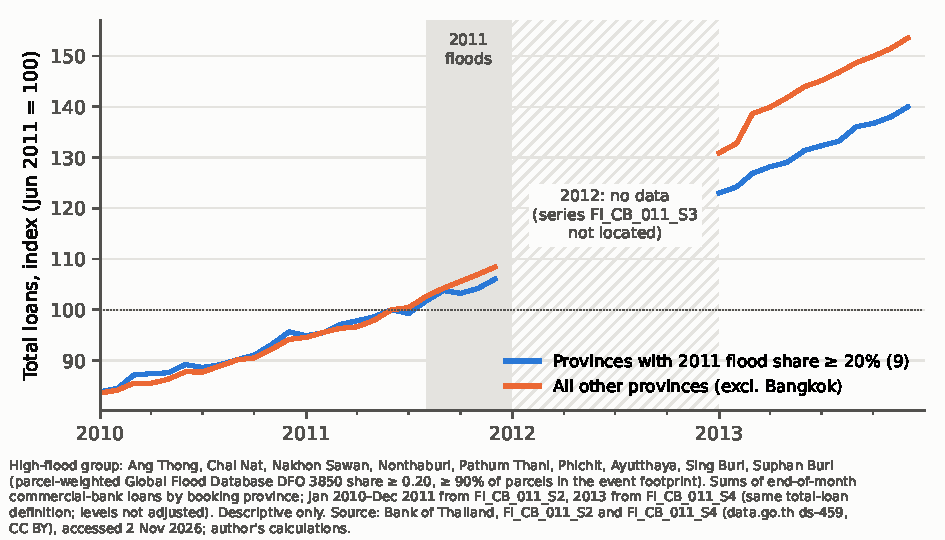
\includegraphics[width=\textwidth]{fig_provincial_credit_2011}
\caption{Commercial-bank loans in the most flooded provinces and elsewhere, 2010--2013}
\label{fig:credit}
\tabnote{Monthly commercial-bank loans by province, Bank of Thailand, indexed to June 2011 \citep{bot2026loansprovince}. ``Flooded'': provinces outside Bangkok with at least 20\% of parcels flooded in the 2011 Global Flood Database event, among provinces with at least 90\% of parcels inside the database footprint; ``other'': all remaining provinces outside Bangkok. The 2012 file of the series was not located, so the \credMissingMonths{} months of 2012 are missing. Source: \texttt{fig\_provincial\_credit\_2011\_data.csv}.}
\end{figure}

Figure~\ref{fig:credit} indexes commercial-bank loans in the provinces where at least a fifth of parcels were flooded in 2011 against the rest of the country outside Bangkok. Loans in the flooded provinces did not fall in level: they stood at \credFloodedDecEleven{} in December 2011 against \credOtherDecEleven{} elsewhere, \credFloodedJanThirteen{} against \credOtherJanThirteen{} in January 2013 and \credFloodedDecThirteen{} against \credOtherDecThirteen{} in December 2013. But they fell behind. From \credPreStart{} to July 2011 the two indices never differed by more than \credPreMaxGap{} points; after the flood the gap is \credGapDecEleven{} points in December 2011, \credGapJanThirteen{} in January 2013 and \credGapDecThirteen{} in December 2013, by which date lending in the flooded provinces was \credRelDecThirteen\% below the other provinces in relative terms. The gap is several times larger than any pre-flood difference, and the flooded provinces never rise above the others after the flood, so there is no sign of the brief credit-demand surge that \citet{albertazzi2026physical} find in the euro area. The series are two aggregates with no counterfactual, the whole of 2012 is missing, and the soft-loan facility of Section~\ref{sec:background} may have substituted for commercial credit, so the shortfall is a description, not an estimate of a flood effect. Provincial credit shares drift slowly: the dissimilarity index of the provincial loan distribution between December 2005 and December 2015 is \driftTenOut{} outside Bangkok and \driftTenWith{} including it, and \driftRecentOut{} and \driftRecentWith{} over 2015--25 (Appendix Table~\ref{tab:drift}). Provincial exposure shares measured today are therefore a reasonable proxy for the shares that would apply over a stress horizon, which Section~\ref{sec:stress} uses.

\begin{table}[t]
\centering\footnotesize
\caption{Appraisal-based residential price index around three floods, relative to other regions}\label{tab:rppi}
% Generated by 04_analysis/src/paper_numbers.py. Do not edit.
\begin{adjustbox}{max width=\textwidth}
\begin{tabular}{llrrrr}
\toprule
Region & Base month & Prior 12 months (\%) & \multicolumn{3}{c}{Change from base month (\%)} \\
\cmidrule(lr){4-6}
 & & & +3 m & +6 m & +10 m \\
\midrule
Bangkok and vicinity & 2011-09 & -- & $-$2.2 & $-$3.4 & $-$7.3 \\
North & 2024-07 & 0.6 & $-$1.2 & $-$0.5 & $-$1.1 \\
South & 2025-10 & 3.3 & 3.1 & 2.2 & 3.2 \\
\bottomrule
\end{tabular}
\end{adjustbox}

\tabnote{Bank of Thailand residential property price index by region, built from lenders' appraisal prices in the mortgage-collateral database \citep{bot2025rppi,bot2026rppislides}. Entries are the region's log change from the base month (the last month before the flood reached the region) minus the mean log change of the other non-Bangkok regions, in per cent. The index is regional, from representative provinces, so most of each region's collateral did not flood; it tracks bank collateral appraisals, not official values. Source: \texttt{rppi\_flood\_windows.csv}.}
\end{table}

Prices show a slow, steady relative decline after 2011. The appraisal-based residential price index is the only public series that bears on bank collateral valuations, although it cannot separate $\lambda_B$ from the discount itself, because it mixes the discount, realised damage and the lenders' valuation behaviour across a whole region. Relative to the other regions, the index for Bangkok and its vicinity fell by \rppiBkkThree\% three months after September 2011, by \rppiBkkSix\% after six and by \rppiBkkTen\% after ten (Table~\ref{tab:rppi}): the fall widened over the ten months the window covers and had not reversed within it. The northern index after the 2024 floods was \rppiNorthThree\% lower at three months and \rppiNorthTen\% at ten, after a \rppiNorthPre\% relative rise over the prior year; the southern index after the 2025 floods kept rising, \rppiSouthTen\% at ten months against \rppiSouthPre\% before. These are regional indices with no treated--control structure and say nothing about the parcels that were flooded; their use is to show that the aggregate appraisal response to the 2011 flood was slow to build and persistent over the window observed, which is what a lagged-valuation mechanism would produce, and also what a slowly realised true loss would produce. Separating the two requires the designs of Sections~\ref{sec:design} and~\ref{sec:credit}.

\subsection{The estimator}

The restricted data would be a monthly loan-level panel with the cadastral sheet of each collateral parcel, days past due, restructuring flags, asset class, stage under TFRS~9, balance and appraised collateral value; the schema is in the replication repository, and the synthetic panel of Appendix~\ref{app:code} is generated to it. The flood exposure of loan $i$ is the radar or optical flood share of its collateral sheet, $\mathrm{Flood}_{s(i)}$, in the event months. For 2011, with the event at October 2011, the specification is an event study with district-by-month effects:
\begin{equation}
y_{it} = \alpha_i + \delta_{d(i),t} + \sum_{q \neq -1} \beta_q\,\mathrm{Flood}_{s(i)}\,\mathbf{1}[q(t) = q] + \varepsilon_{it},
\label{eq:es}
\end{equation}
where $q(t)$ is the quarter relative to the event, binned at $-4$ and $+6$, and $y$ is default (more than 90 days past due), restructuring, stage~2, or distress (default or restructuring). The relief rules enter through a triple difference: $e_i$ indicates that the loan was Normal or Special Mention in September 2011 and hence eligible for the classification freeze, and the specification adds $\sum_q \theta_q\,\mathrm{Flood}_{s(i)}\,e_i\,\mathbf{1}[q(t)=q]$ with eligibility-by-month effects. The effect of flooding on eligible loans is $\beta_q + \theta_q$, on ineligible loans $\beta_q$, and $\theta_q$ in the default equation measures the censoring. Fixed effects are removed by alternating projections and standard errors are clustered by district. The reported quantity is the average of the quarterly coefficients over the four quarters from October 2011 to September 2012, the period in which the classification freeze and the revaluation deferral were in force.

For 2024 and 2025 the same specification applies with the Sentinel-1 flood share, the declared-zone and Level-4 boundaries providing the eligibility variation, and stage~2 as an outcome that did not exist in 2011. The separation of \emph{flooded} from \emph{declared} is the key to telling the flood effect from the relief effect: the satellite maps flooding, the administrative lists define relief, and the two do not coincide. On a synthetic panel in which prediction P3 holds by construction, the estimator recovers the planted distress effect, the censoring of default among eligible loans and its re-routing into restructuring and stage~2 (Appendix Table~\ref{tab:rq2synth}); that is a test of the code, not of the world.

\subsection{Sample sizes}

\begin{table}[t]
\centering\footnotesize
\caption{Flooded borrowers needed to detect a flood effect on distress, 2024--25 design}\label{tab:rq2power}
% Generated by 04_analysis/src/paper_numbers.py. Do not edit.
\begin{adjustbox}{max width=\textwidth}
\begin{tabular}{llrrrrr}
\toprule
Base rate & Design effect & \multicolumn{3}{c}{Flooded borrowers needed for} & \multicolumn{2}{c}{MDE (pp) with} \\
\cmidrule(lr){3-5}\cmidrule(lr){6-7}
 & & 0.7 pp & 1 pp & 2 pp & 1,000 & 2,000 \\
\midrule
3 & 1.5 & 8,740 & 4,283 & 1,071 & 2.07 & 1.46 \\
3 & 2.0 & 11,654 & 5,711 & 1,428 & 2.39 & 1.69 \\
5 & 1.5 & 14,267 & 6,991 & 1,748 & 2.64 & 1.87 \\
5 & 2.0 & 19,022 & 9,321 & 2,331 & 3.05 & 2.16 \\
\bottomrule
\end{tabular}
\end{adjustbox}

\tabnote{Two-sided test at 5\% with 80\% power of a difference in twelve-month distress rates between flooded and unflooded borrowers, four controls per flooded borrower, with the design effect capturing clustering by collateral sheet. Base rate: twelve-month distress rate among unflooded borrowers. Source: \texttt{rq2\_power\_2024.csv}.}
\end{table}

Table~\ref{tab:rq2power} gives the sample sizes the 2024--25 design needs. With a base twelve-month distress rate of 3\% and a design effect of 1.5, detecting a 1~percentage-point rise needs \rqTwoNeedOne{} flooded borrowers, a 2-point rise \rqTwoNeedTwo, and the 0.7-point effect that \citet{albertazzi2026physical} find needs \rqTwoNeedLow{} (\rqTwoNeedLowPess{} under a 5\% base rate and a design effect of 2). With 1,000 flooded borrowers the minimum detectable effect is \rqTwoMdeThousand{} points, with 2,000 it is \rqTwoMdeTwoThousand. For the 2011 event, where the interest is in whether relief equalised outcomes, an equivalence test with a 5-point margin on a continuous distress score with standard deviation 0.3, a first stage of 0.75 and a design effect of 1.5 needs \rqTwoEquivN{} loans per group, and \rqTwoEquivNBest{} under the most favourable assumptions (Appendix Table~\ref{tab:rq2equiv}). A single mid-sized bank's retail book in the flooded provinces would meet the 2024--25 requirement; the 2011 equivalence design needs a credit-bureau-scale sample.

If loan-level access is not granted, the fallback is weaker and uses public data only: the staging, restructuring and relief disclosures of listed banks around the flood years, combined with the provincial aggregates above and with the exposure mapping of \citet{worldbank2026ccdrfin}. It can show whether stage~2 shares rose for the most exposed banks, as \citet{perezmontes2025impact} find in Spain, but not the collateral-level mechanism.
